\clearpage
\section{Raw results from the U.S. complementary surveys (US1 and US2)}\label{app:raw_results_US}

\begin{figure}[h!]
    \caption{Correct answers to comprehension questions. (Questions \ref{q:understood_gcs}-\ref{q:understood_both})}\label{fig:understood_each}
    \makebox[\textwidth][c]{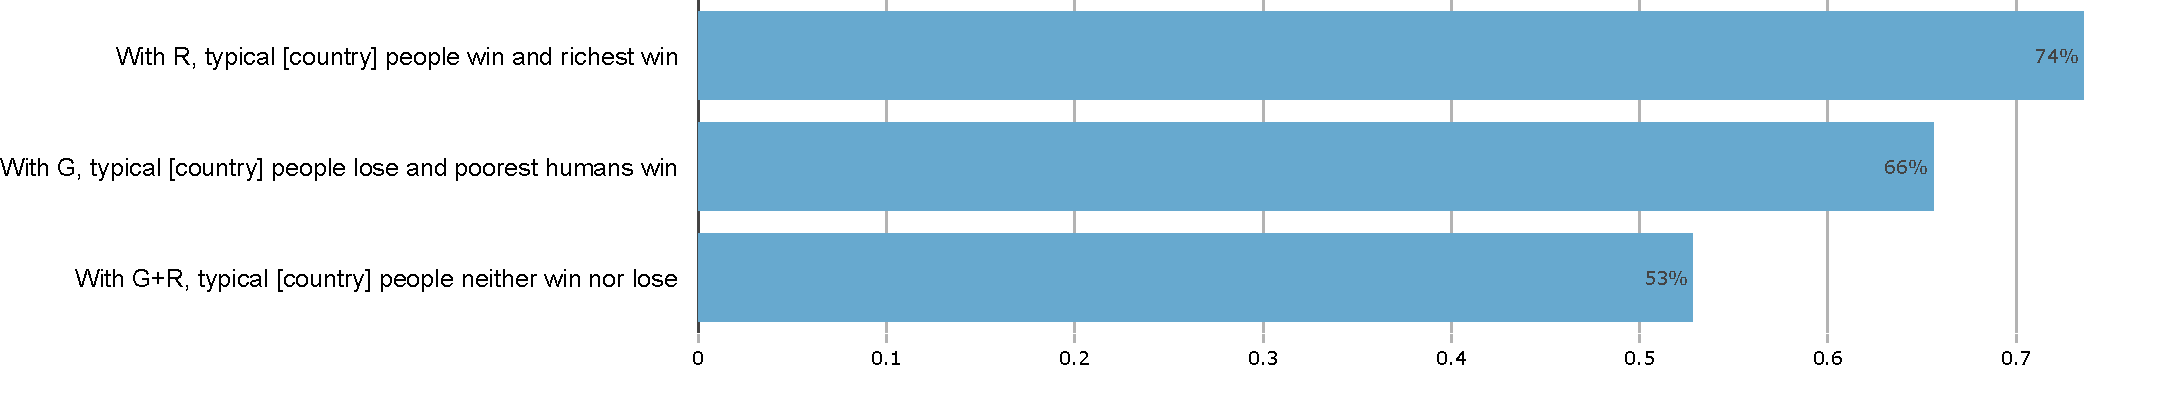
\includegraphics[width=\textwidth]{../figures/US1/understood_each.pdf}} 
\end{figure}

\begin{figure}[h!]
    \caption{Number of correct answers to comprehension questions. (Questions \ref{q:understood_gcs}-\ref{q:understood_both})}\label{fig:understood_score}
    \makebox[\textwidth][c]{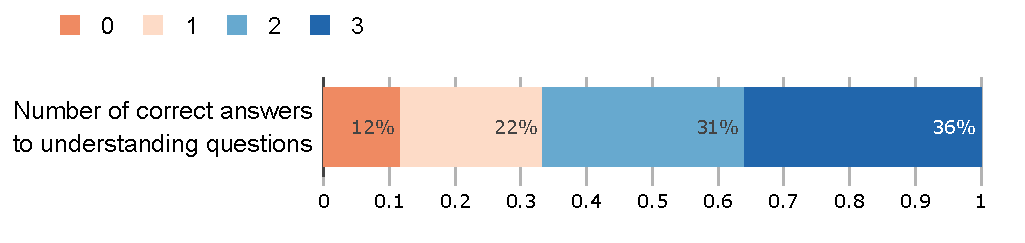
\includegraphics[width=.8\textwidth]{../figures/US1/understood_score.pdf}} 
\end{figure}

\begin{figure}[h!]
    \caption{Support for the GCS, NC and the combination of GCS, NR and C. (Questions \ref{q:gcs_support}, \ref{q:nr_support} and \ref{q:crg_support})}\label{fig:support_binary}
    \makebox[\textwidth][c]{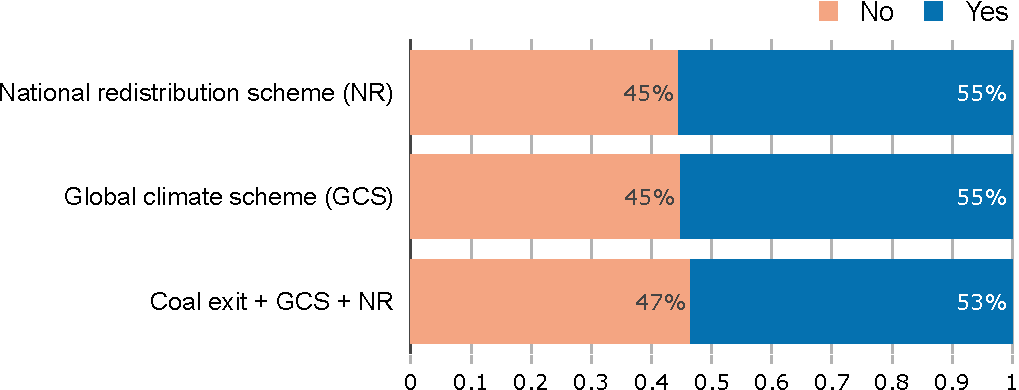
\includegraphics[width=.9\textwidth]{../figures/US1/support_binary.pdf}} 
\end{figure}

\begin{figure}[h!]
    \caption{Beliefs regarding the support for the GCS and NR. (Questions \ref{q:gcs_belief} and \ref{q:nr_belief})}\label{fig:belief}
    \makebox[\textwidth][c]{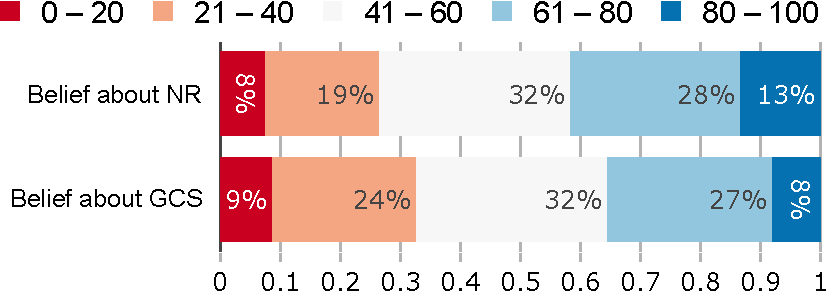
\includegraphics[width=.8\textwidth]{../figures/US1/belief.pdf}} 
\end{figure}

\begin{figure}[h!]
    \caption{List experiment. (Question \ref{q:list_exp})}\label{fig:list_exp}
    \makebox[\textwidth][c]{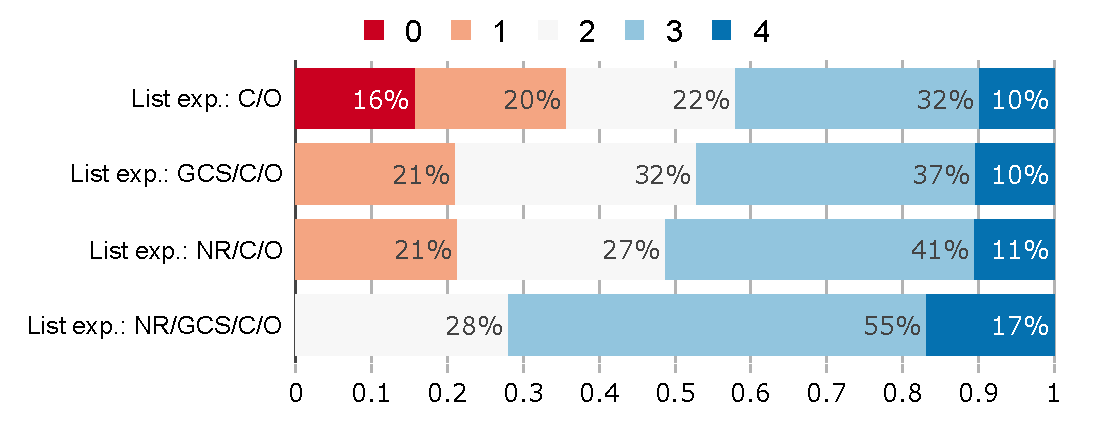
\includegraphics[width=.8\textwidth]{../figures/US1/list_exp.pdf}} 
\end{figure}

\begin{figure}[h!]
    \caption{Conjoint analyses. (Questions \ref{q:conjoint_a}-\ref{q:conjoint_d})}\label{fig:conjoint}
    \makebox[\textwidth][c]{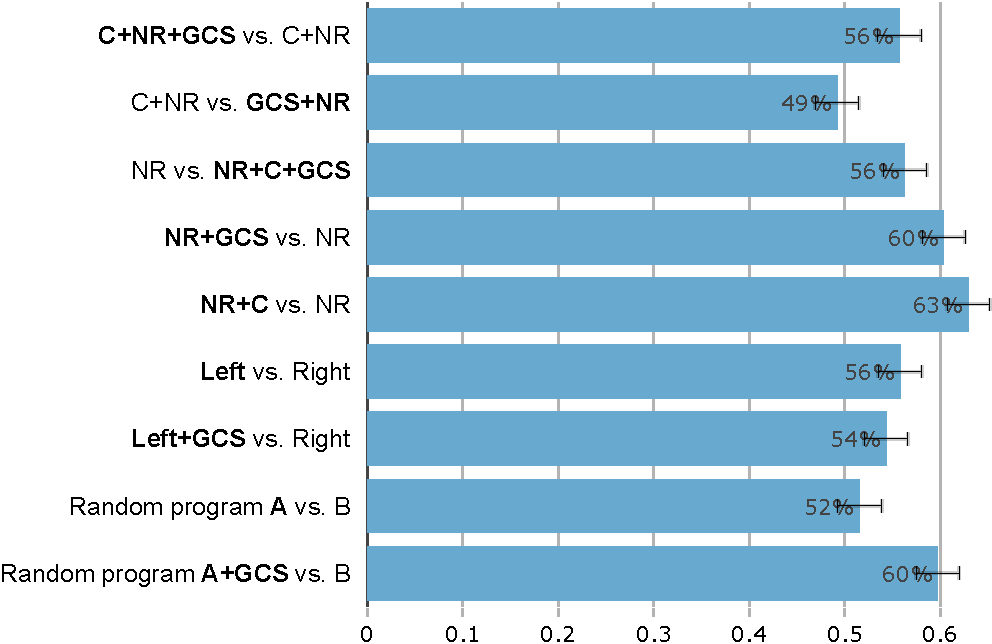
\includegraphics[width=\textwidth]{../figures/US1/conjoint.pdf}} 
\end{figure}

\begin{figure}[h!] % already in text
    \caption{[Asked only to non-Republicans] Conjoint analysis n°4: random programs at the Democratic primary. (Question \ref{q:conjoint_r})}\label{fig:ca_r}
    \makebox[\textwidth][c]{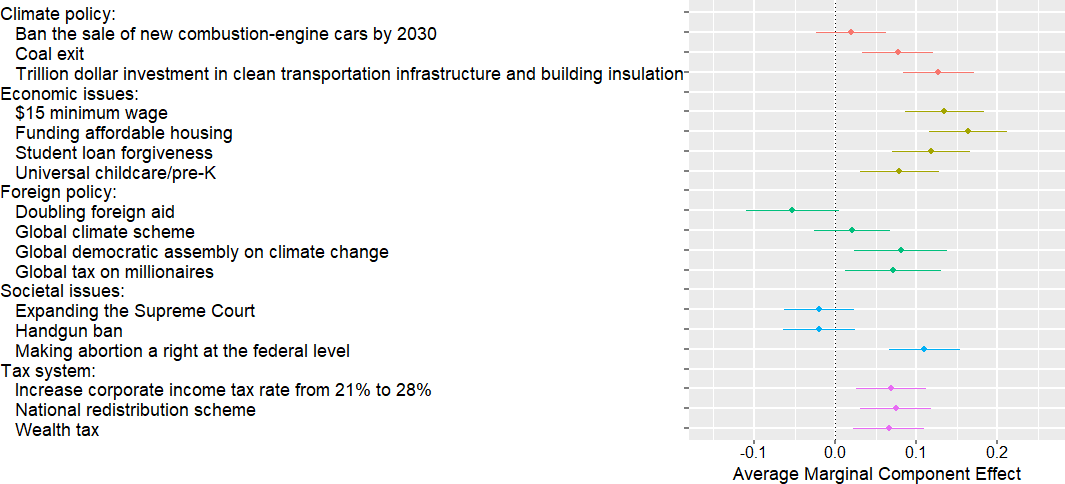
\includegraphics[width=\textwidth]{../figures/US1/ca_r.png}} 
\end{figure}

\begin{figure}[h!]
    \caption{Donation in case of lottery win. (Question \ref{q:donation})}\label{fig:donation}
    \makebox[\textwidth][c]{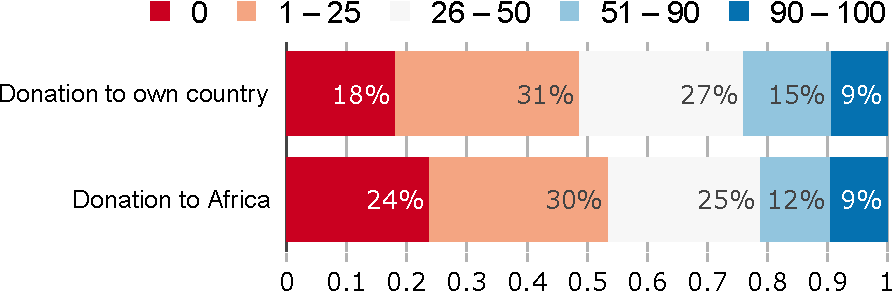
\includegraphics[width=.8\textwidth]{../figures/US1/variables_donation.pdf}} 
\end{figure}

\begin{figure}[h!]
    \caption{Willingness to sign real-stake petition for the GCS or NR. (Question \ref{q:petition})}\label{fig:petition}
    \makebox[\textwidth][c]{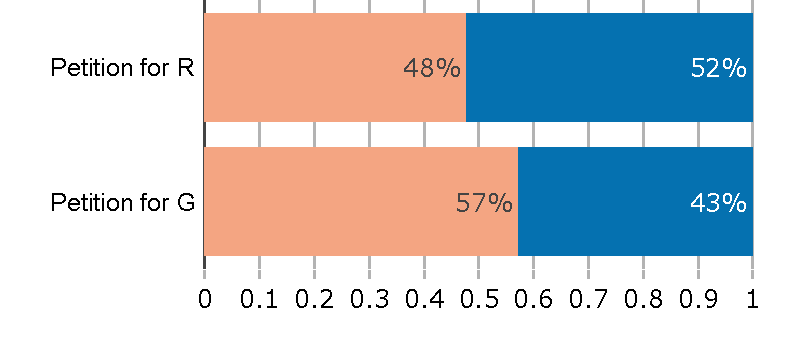
\includegraphics[width=.7\textwidth]{../figures/US1/variables_petition.pdf}} 
\end{figure}

\begin{figure}[h!] % already in text
    \caption{Support for various global policies. (Questions \ref{q:climate_policies} and \ref{q:other_policies})}\label{fig:support_likert}
    \makebox[\textwidth][c]{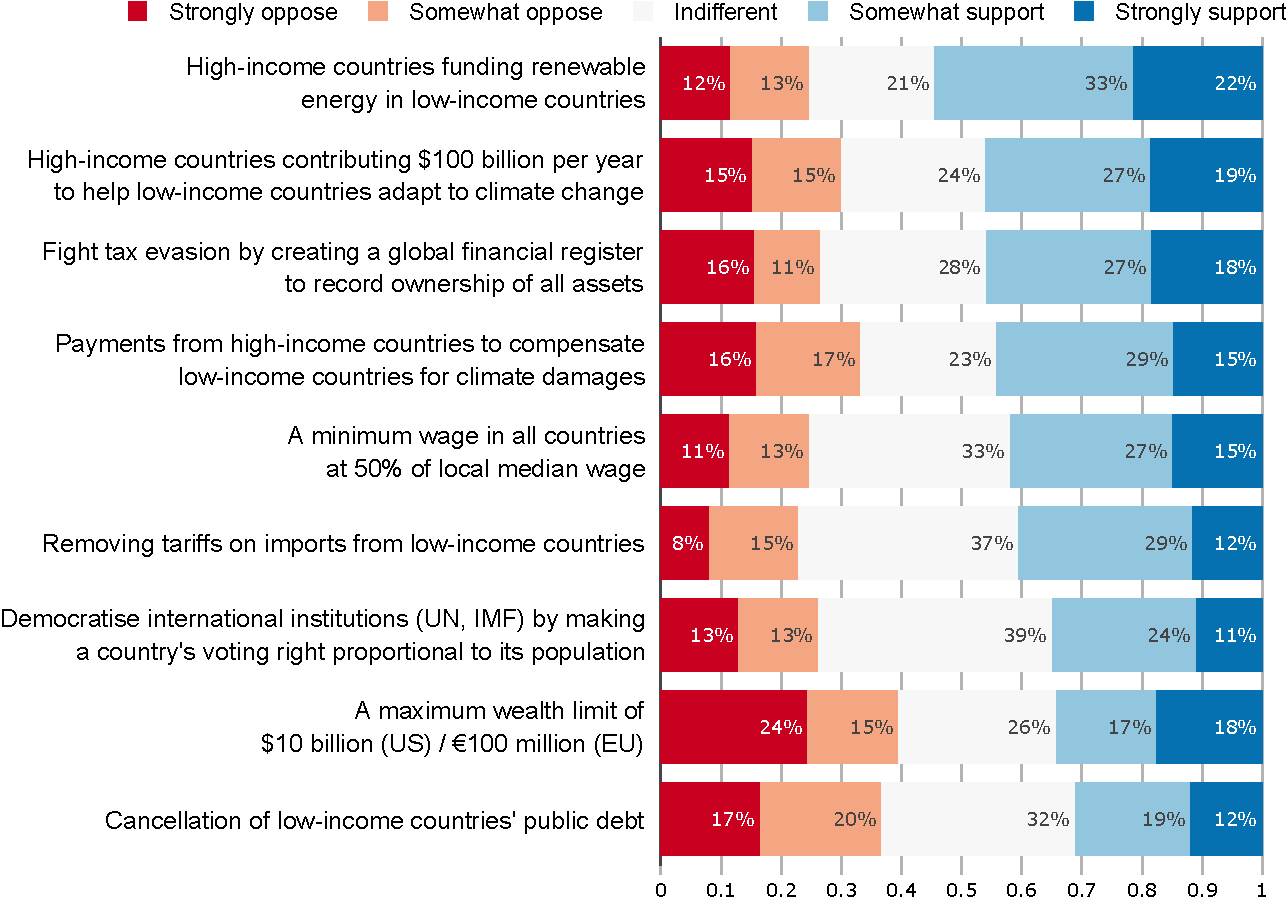
\includegraphics[width=\textwidth]{../figures/US1/support_likert.pdf}} 
\end{figure}

% \begin{figure}[h!]
%     \caption{label}\label{fig:climate_policies}
%     \makebox[\textwidth][c]{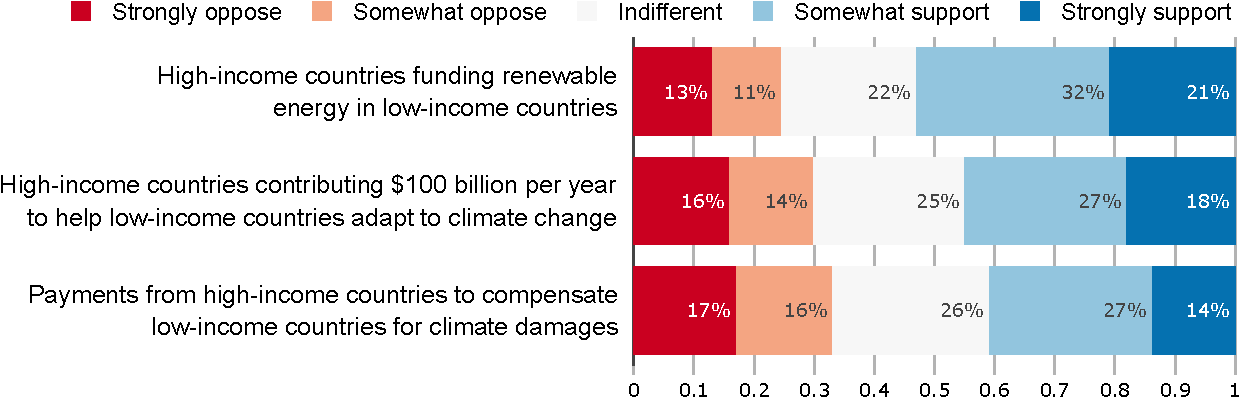
\includegraphics[width=\textwidth]{../figures/US1/climate_policies.pdf}} 
% \end{figure}

% \begin{figure}[h!]
%     \caption{label}\label{fig:global_policies}
%     \makebox[\textwidth][c]{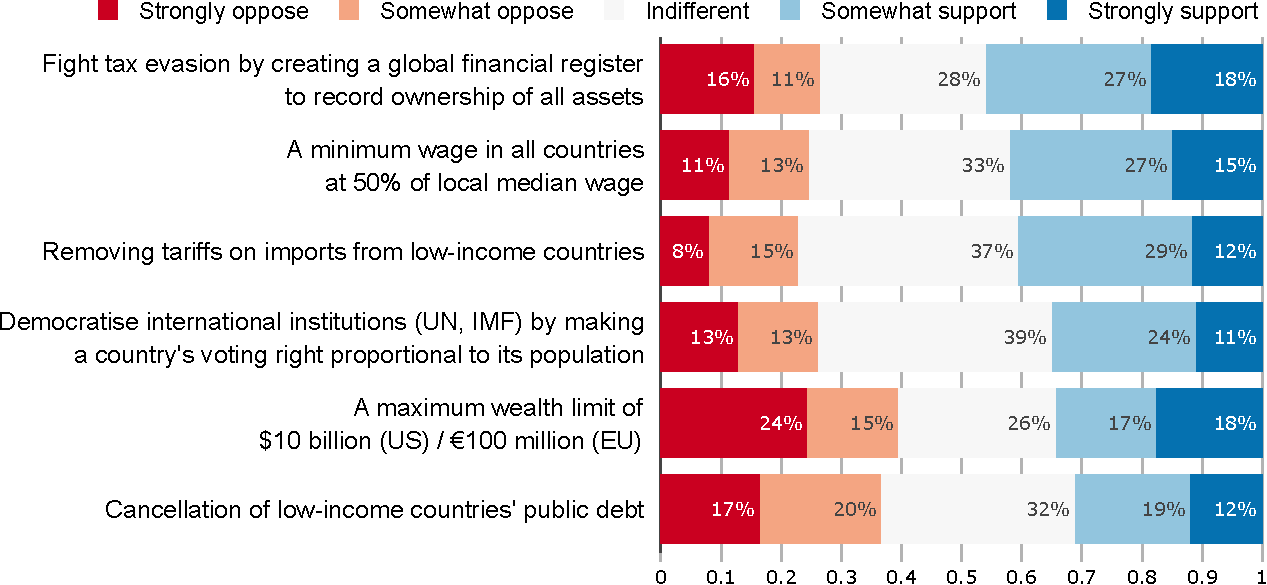
\includegraphics[width=\textwidth]{../figures/US1/global_policies.pdf}} 
% \end{figure}

\begin{figure}[h!]
    \caption{Attitudes regarding the evolution of U.S. foreign aid. (Question \ref{q:foreign_aid_raise_support})}\label{fig:foreign_aid_raise_support}
    \makebox[\textwidth][c]{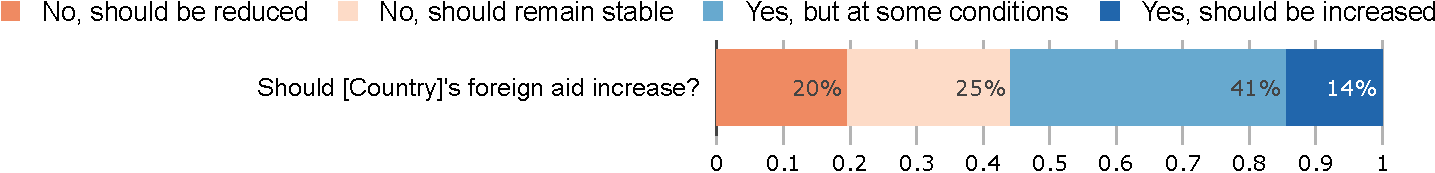
\includegraphics[width=\textwidth]{../figures/US1/foreign_aid_raise_support.pdf}} 
\end{figure}

\begin{figure}[h!]
    \caption{[Asked to those who wish an increase of foreign aid at some conditions.] Conditions at which foreign aid should be increased. (Question \ref{q:foreign_aid_condition})}\label{fig:foreign_aid_condition}
    \makebox[\textwidth][c]{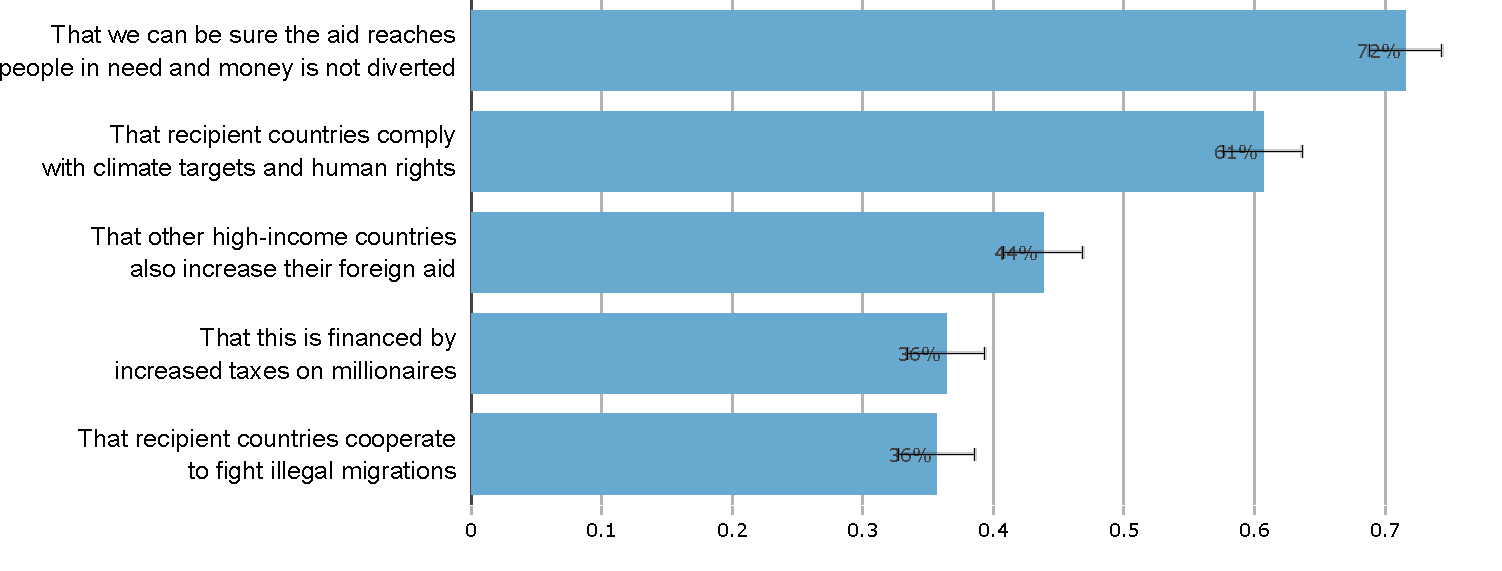
\includegraphics[width=\textwidth]{../figures/US1/foreign_aid_condition.pdf}} 
\end{figure}

\begin{figure}[h!]
    \caption{[Asked to those who wish a decrease or stability of foreign aid.] Reasons why foreign aid should not be increased. (Question \ref{q:foreign_aid_no})}\label{fig:foreign_aid_no}
    \makebox[\textwidth][c]{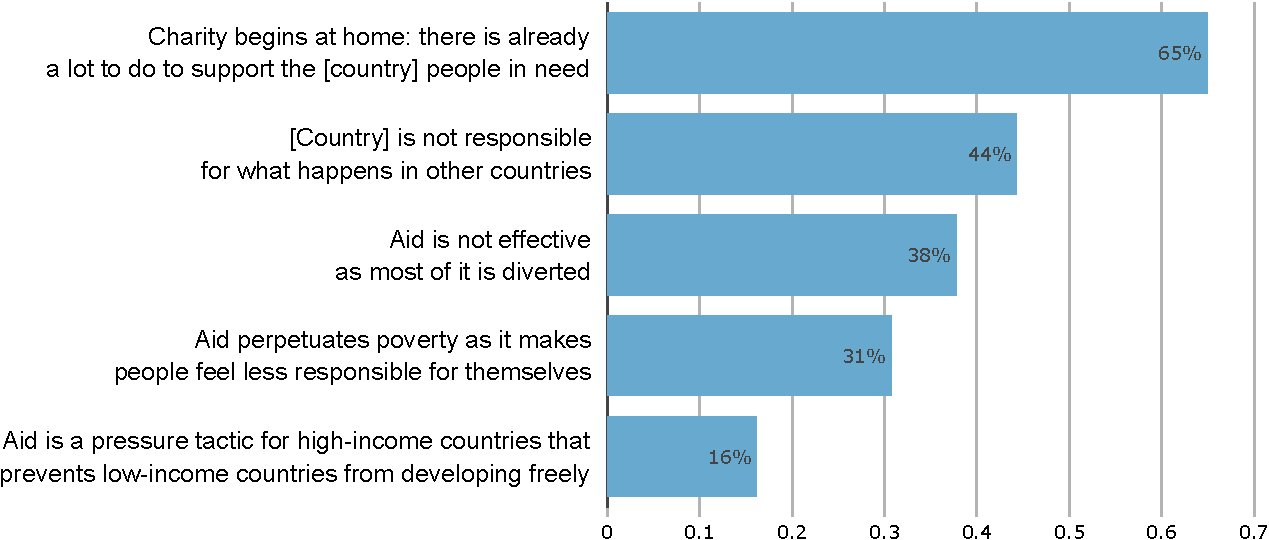
\includegraphics[width=\textwidth]{../figures/US1/foreign_aid_no.pdf}} 
\end{figure}

\begin{figure}[h!]
    \caption{Preferred approach of U.S. diplomats at international climate negotiations. (Question \ref{q:negotiation})}\label{fig:negotiation}
    \makebox[\textwidth][c]{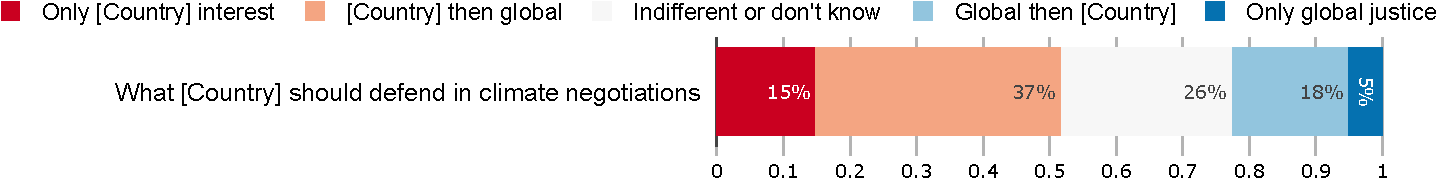
\includegraphics[width=\textwidth]{../figures/US1/negotiation.pdf}} 
\end{figure}

% \begin{figure}[h!]
%     \caption{label}\label{fig:vote}
%     \makebox[\textwidth][c]{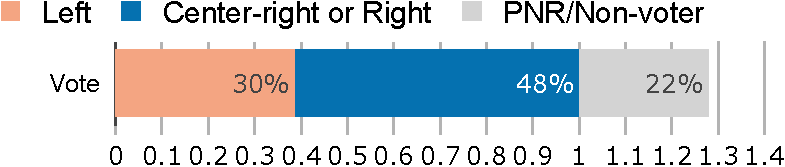
\includegraphics[width=\textwidth]{../figures/US1/vote.pdf}} 
% \end{figure}

\begin{figure}[h!]
    \caption{Extent to which selected issues are viewed as important problems. (Question \ref{q:problem})}\label{fig:problem}
    \makebox[\textwidth][c]{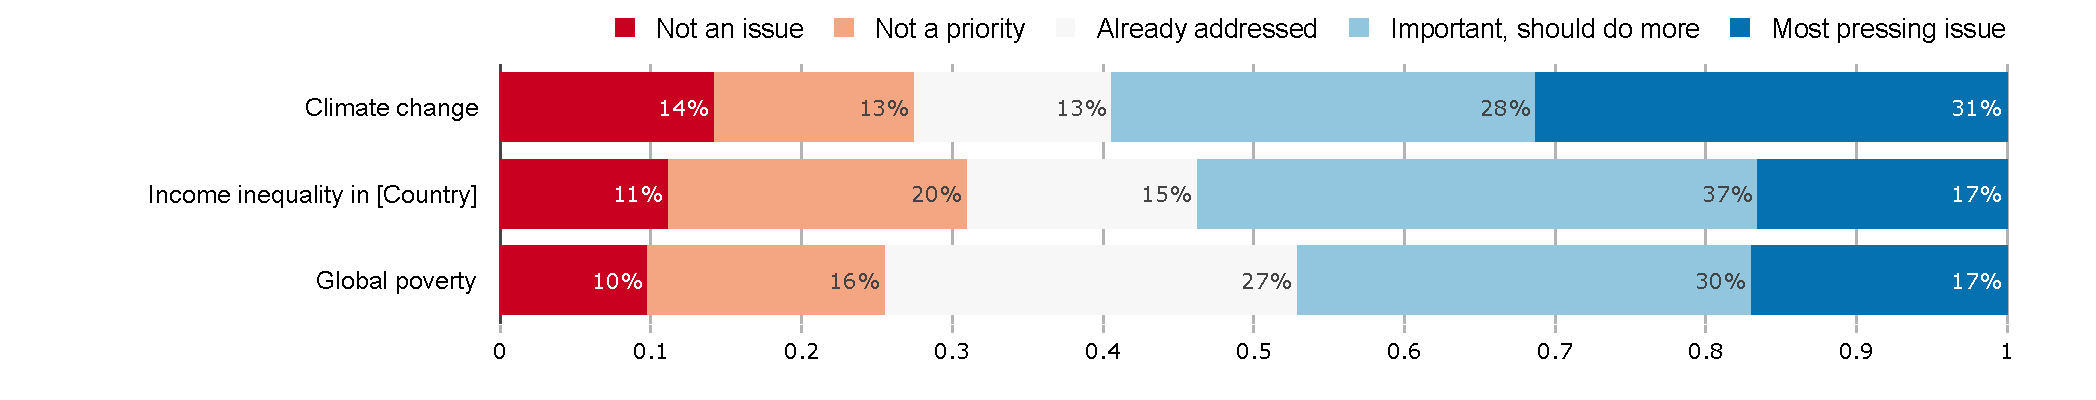
\includegraphics[width=\textwidth]{../figures/US1/problem.pdf}} 
\end{figure}

\begin{figure}[h!]
    \caption{Group defended when voting. (Question \ref{q:group_defended_agg})}\label{fig:group_defended_agg2}
    \makebox[\textwidth][c]{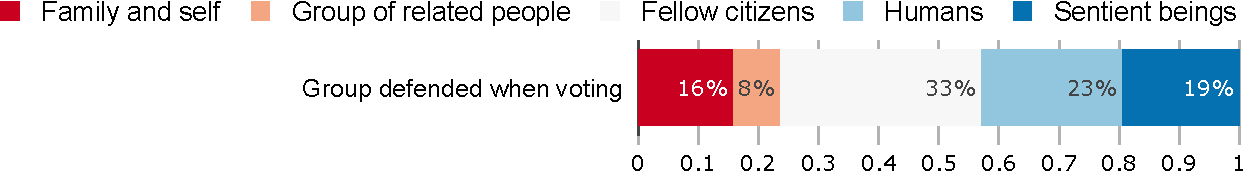
\includegraphics[width=\textwidth]{../figures/US1/group_defended_agg2.pdf}} 
\end{figure}

% \begin{figure}[h!]
%     \caption{label}\label{fig:group_defended}
%     \makebox[\textwidth][c]{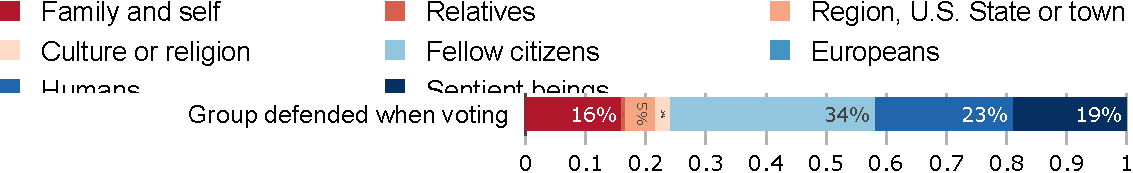
\includegraphics[width=\textwidth]{../figures/US1/group_defended.pdf}} 
% \end{figure}

\begin{figure}[h!] % already in text
    \caption{Prioritization of policies. (Question \ref{q:points_us})}\label{fig:points_us}
    \makebox[\textwidth][c]{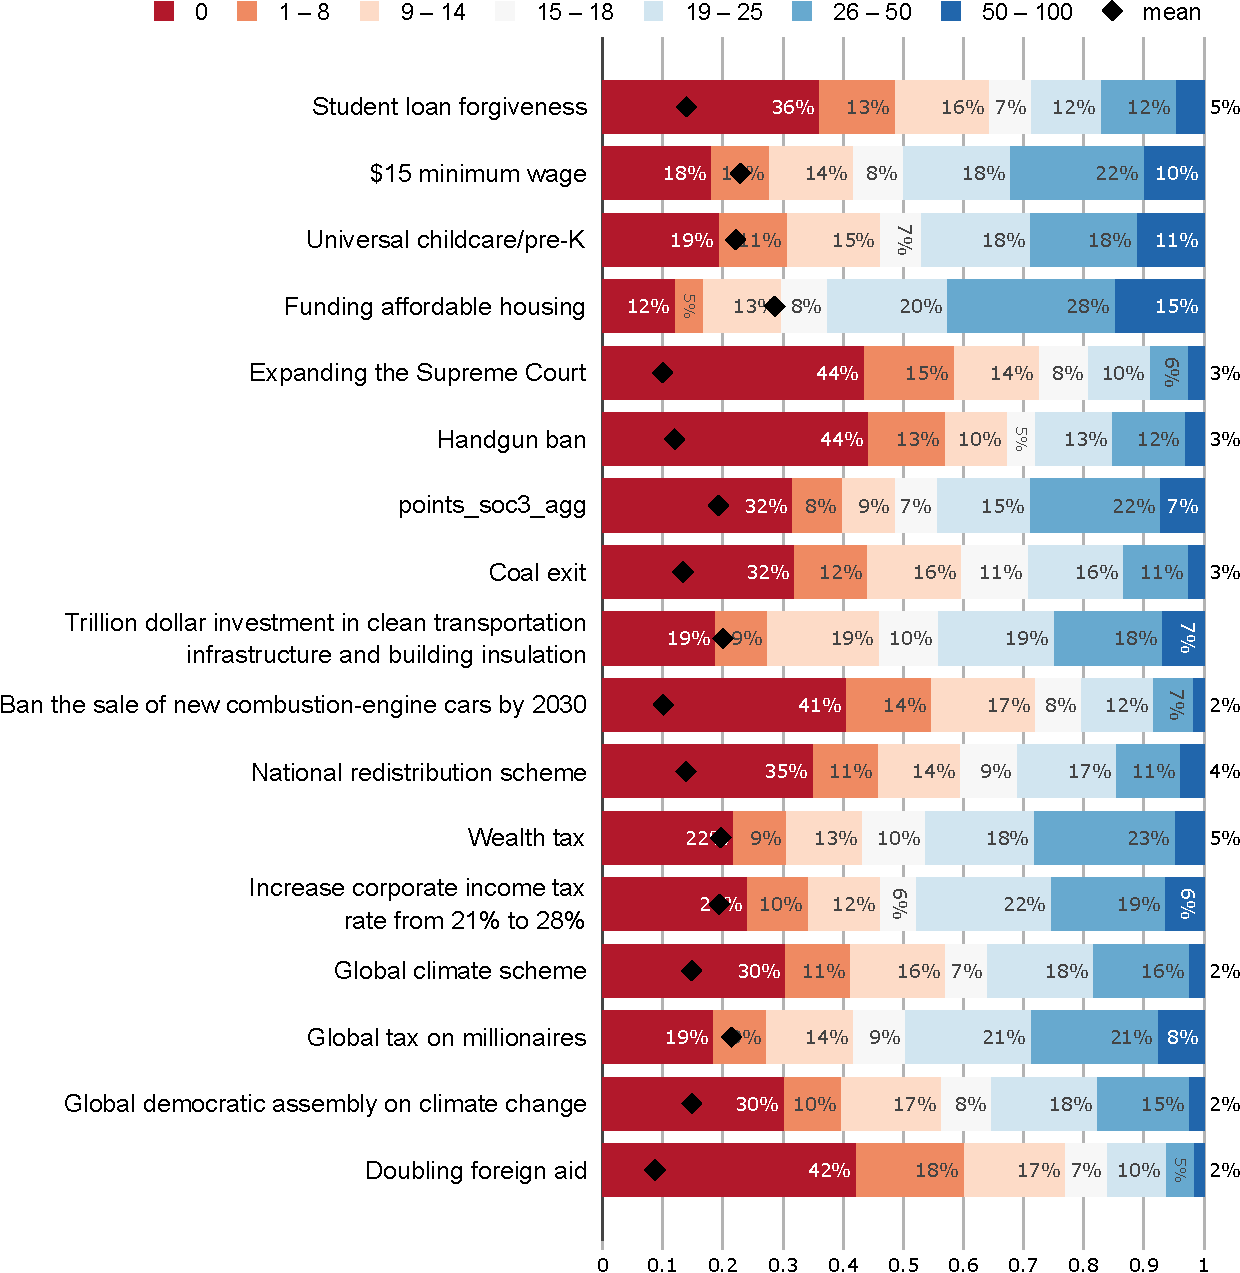
\includegraphics[width=\textwidth]{../figures/US1/points_mean.pdf}} 
\end{figure}

% \begin{figure}[h!]
%     \caption{label}\label{fig:share_policies_supported}
%     \makebox[\textwidth][c]{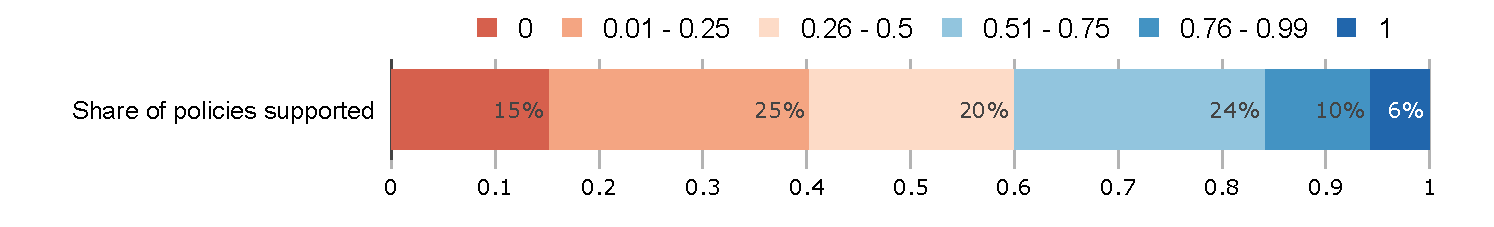
\includegraphics[width=\textwidth]{../figures/US1/share_policies_supported.pdf}} 
% \end{figure} % TODO? uncomment?

% \begin{figure}[h!]
%     \caption{label}\label{fig:vars}
%     \makebox[\textwidth][c]{\includegraphics[width=\textwidth]{../figures/US1/vars.pdf}} 
% \end{figure}
